\newpage

\chapter{実験}

本章では,3章において提案されたシステムの評価実験について述べる.まず,実験に関する具体的な設定と定性評価のためのアンケート項目を示す.その後,実験結果について定性,定量の順で考察を交えつつ述べ,最後に提案システムの評価を総括する.

\section{実験方法}
提案システムを評価するために,20代から30代の男女計11人(男9人,女2人)にユーザ実験の協力をしていただいた.また,被験者の中で Blender などの DCC ツールの経験があるのは6人であった.提案システムと対照実験用のシステムに対して,二つのモデリングタスクを行った後,使用感に関するアンケートに答えてもらった.

二つのモデリングタスクは予め用意した画像に近づけるようにモデリングしてもらうタスクと,ユーザが満足するまで完全に自由にモデリングをしてもらうタスクである.それぞれの意図として,コンテンツ制作には多人数で行う場合と個人で行う場合とがあり,多人数で行うときには予め完成イメージを共有したうえで行うのに対して,個人での場合は制約なく行うからであり,二つのタスクはこの2パターンの簡易的な再現を行っている.

本実験における評価について,システム操作時間とプロシージャルモデリングのパラメータ変化による定量評価および,アンケートによる定性評価から提案システムの有意性について議論を行う.

\subsection{実験環境}
本提案手法では,3DCGのモデリングを実験するにあたり,複数のオブジェクトを同時に見ることや,変形における動作ラグが予測される.まず,表\ref{tb:pcEnv}システム使用時のPC環境を以下に示す.
\begin{table}[h]
	\centering
	\caption{PC 環境\label{tb:pcEnv}}
	\scalebox{1.0}{
		\begin{tabular}{|c||c|} \hline
                OS&Windows 11 Home\\ \hline
			CPU&12th Gen intel(R) Core(TM) i7-12700\\ \hline
                RAM&32GB\\ \hline
			GPU&NVIDIA GeForce RTX 3080\\ \hline\
			画面サイズ&27inch\\ \hline
                解像度&2560$\times$1440\\ \hline\hline
			ソフト&Blender 3.6.7\\ \hline
		\end{tabular}
	}
\end{table}
\subsection{実験設定}
実験設定について,二種類のモデリングタスクおよび,対照実験について説明する.

\subsubsection{実験1}
実験1では,あらかじめ制作された目標モデルの画像を見て,それに近いモデルを作ってもらうタスクを設定した.対象とするモデルは HuyKhoi2407 によって作成された Procedural Cake \footnote[4]{\url{https://blendermarket.com/products/procedural-cake--blender-geometry-nodes} } で,パラメータ数は11である.以降 Cake モデルと呼ぶ.表\ref{tb:cakeParam}にパラメータの名前,data type,範囲 および制作してもらう目標モデルのパラメータを示す.また,図\ref{fig:cake1}に実際に被験者に参考にしてもらった画像について示す.パラメータの名前からも分かる通り,ケーキについてカットする角度や,ホール,クリームなどの大きさ,トッピングの数や皿の状態を指定する事が出来る.本モデルを選んだ理由として,パラメータを動かしたときにモデルの外観との対応が非常に分かりやすく,パラメータ数が11と比較的少ないことが挙げられる.また,実際にパラメータが最大最小を取るときの外観について\hyperref[paramMean]{付録A}に掲載する.

\begin{table}[h]
	\centering
	\caption{Cake モデルのパラメータ\label{tb:cakeParam}}
	\scalebox{1.0}{
		\begin{tabular}{|c|c|c|c||c|} \hline
                name&data type&min&max&目標モデル\\ \hline\hline
			Cake cut&Float&0.0&1.0&0.782\\ \hline
                Cake height&Float&0.5&2.0&1.03\\ \hline
                Cake radius&Float&0.5&2.0&1.00\\ \hline
                Topping quantity&Float&0.0&50.0&41.3\\ \hline
                Topping position&Float&0.0&1.0&0.314\\ \hline
                CreamBot quantity&Float&0.0&50.0&29.2\\ \hline
                CreamBot Size&Float&0.0&2.0&1.46\\ \hline
                CreamTop quantity&Float&0.0&50.0&15.9\\ \hline
                CreamTop Size&Float&0.0&2.0&0.900\\ \hline
                Plate size&Float&0.3&1.0&0.645\\ \hline
                Plate thickness&Float&-0.2&-0.1&-0.159\\ \hline
                
		\end{tabular}
	}
\end{table}


\begin{figure}
\vspace{-2cm}
\centering
\begin{tabular}{c}
  \begin{minipage}{.7\linewidth}
    \centering
    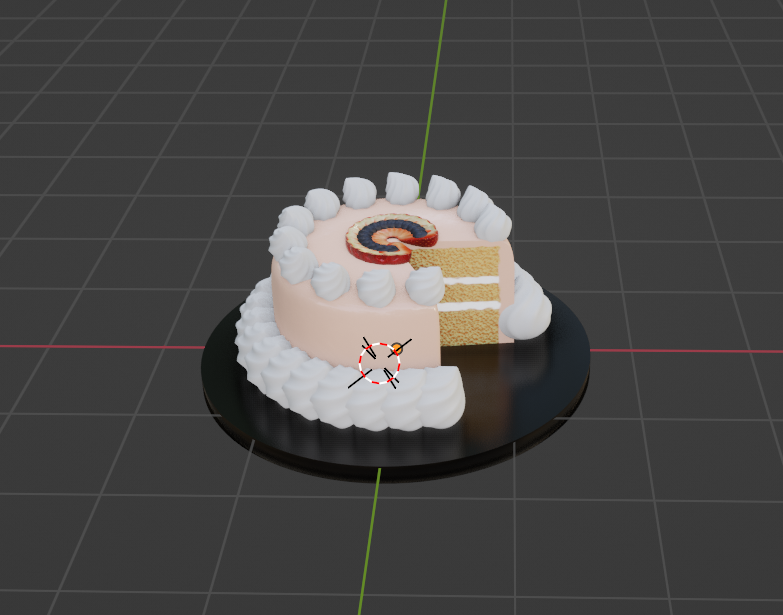
\includegraphics[scale=0.45]{./imgs/cakeSample/cake1.png}
    \subcaption{正面}
  \end{minipage}\\ 
  \begin{minipage}{.7\linewidth}
    \centering
    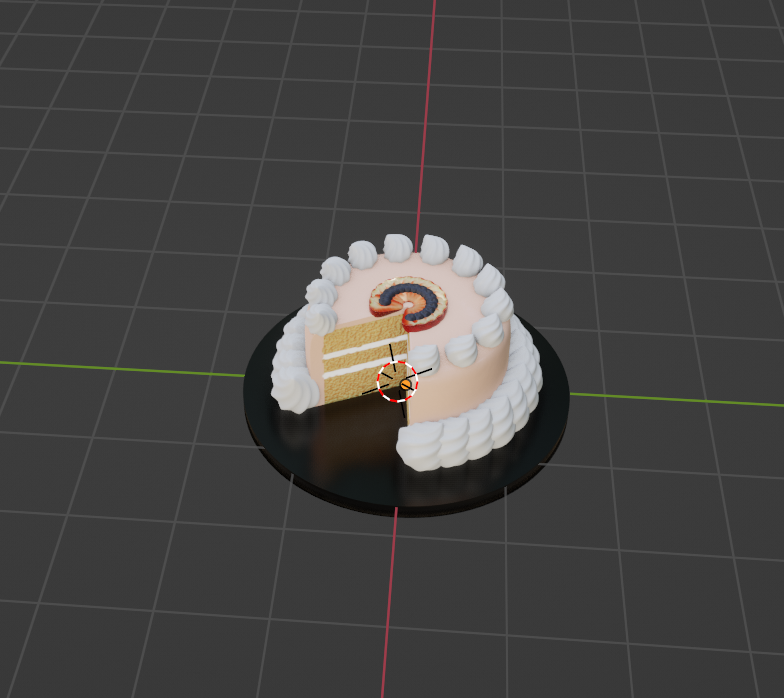
\includegraphics[scale=0.45]{./imgs/cakeSample/cake2.png}
    \subcaption{右}
  \end{minipage}\\ 
  \begin{minipage}{.7\linewidth}
    \centering
    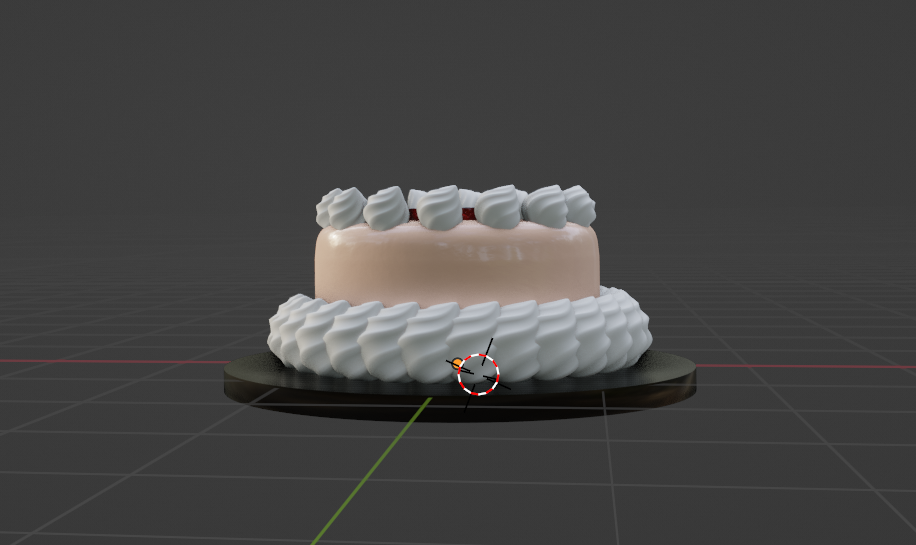
\includegraphics[scale=0.4]{./imgs/cakeSample/cake3.png}
    \subcaption{背面}
  \end{minipage}
\end{tabular}
\caption{目標の Cake モデルの外観}\label{fig:cake1}
\end{figure}

\clearpage
\newpage

\subsubsection{実験2}
実験2では,実験1のような明確な目的を用意せずに自由にモデリングを行ってもらうタスクを設定した.対象とするモデルは Blender Bash によって作成された Procedural Furniture Chair - Sofa - Table - Bed \footnote[5]{\url{https://blendermarket.com/products/procedural-furniture-chair---sofa---table---bed} }で,パラメータ数は25とある程度大きなモデルを利用する.以降 Sofa モデルと呼ぶ.表\ref{tb:sofaParam}にパラメータの名前, data type, 範囲を示す.図\ref{fig:sofa1}に Sofa モデルの一例について示す.また,実際にパラメータが最大最小値を取るときの外観について\hyperref[paramMean]{付録A}に掲載する.パラメータ名に
"NO / 1 / YES"とあるものは,本体のモデルの横に,壁あるいはクッションを付属するためのパラメータであり,パラメータが0(= NO)の時は何もなし,1はモデルの正面向かって左側のみに,2(= YES)の時は両側につけるものとなっている.

\begin{figure}[h]
\centering
\begin{tabular}{c}
  \begin{minipage}{.7\linewidth}
    \centering
    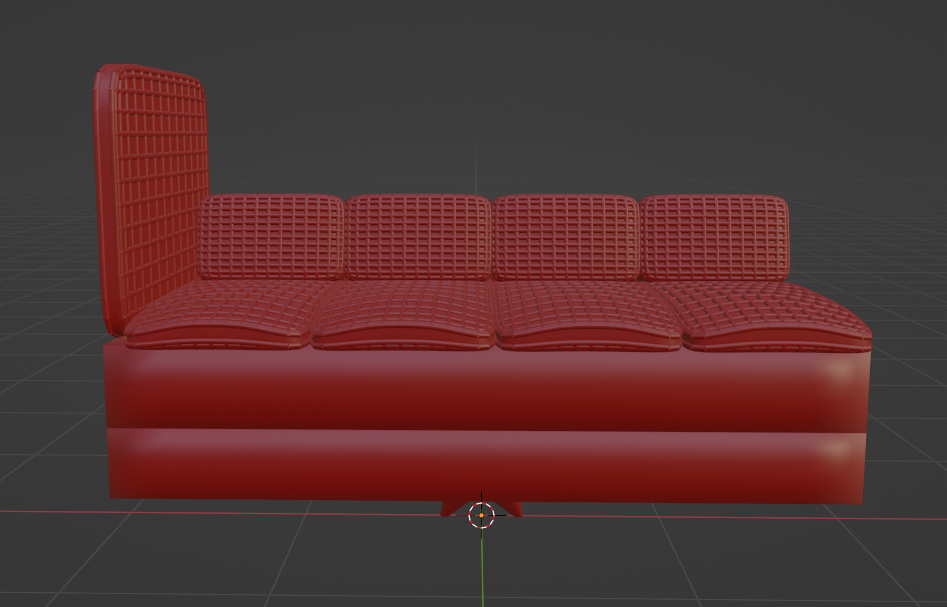
\includegraphics[scale=0.27]{./imgs/sofaSample/sofa1.png}
    \subcaption{正面}
  \end{minipage}\\ \\
  \begin{minipage}{.7\linewidth}
    \centering
    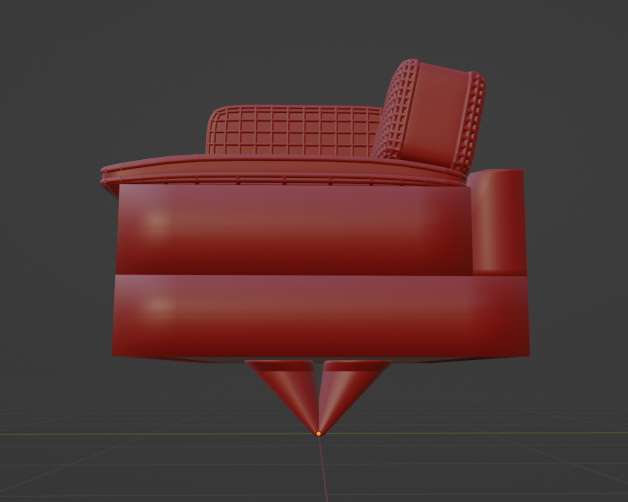
\includegraphics[scale=0.35]{./imgs/sofaSample/sofa2.png}
    \subcaption{右}
  \end{minipage}
\end{tabular}
\caption{sofa モデルの一例}\label{fig:sofa1}
\end{figure}

\begin{table}[h]
	\centering
	\caption{Sofa モデルのパラメータ\label{tb:sofaParam}}
	\scalebox{1.0}{
		\begin{tabular}{|c|c|c|c|} \hline
                name&data type&min&max\\ \hline\hline
			Depth&Float&0.2&4.0\\ \hline
                Width&Float&0.3&5.0\\ \hline\hline
                Legs height&Float&0.01&1.0\\ \hline
                Leg shape&Float&0.0&20.0\\ \hline
                Leg diameter&Float&0.01&0.04\\ \hline
                Leg angle&Float&0.0&1.0\\ \hline
                Leg position&Float&0.02&5.0\\ \hline\hline
                Base height&Float&0.01&0.5\\ \hline
                Base2 height&Float&0.01&0.5\\ \hline\hline
                Back thickness&Float&0.01&0.3\\ \hline
                Back/Side height&Float&0.01&1.5\\ \hline\hline
                Side NO / 1 / YES&Int&0&2\\ \hline
                Side thickness&Float&0.02&0.03\\ \hline\hline
                N. of Cushions&Int&0&5\\ \hline
                Cushion thickness&Float&0.05&0.5\\ \hline
                Cushion nosing&Float&0.0&0.3\\ \hline\hline
                Back Cushion height&Float&0.1&0.7\\ \hline
                Back Cush. Thickness / *Puffiness&Float&0.05&0.5\\ \hline\hline
                Side Cushions NO / 1 / YES&Int&0&2\\ \hline
                Side Cushion Height&Float&0.1&1.8\\ \hline
                Side Cushion Thickness&Float&0.05&0.5\\ \hline\hline
                Cushion Stitching&Float&0.0&0.05\\ \hline
                Cushion Crease&Float&0.0&0.3\\ \hline
                Bevel&Float&0.001&1.0\\ \hline
                Subd&Int&0&2\\ \hline
                
		\end{tabular}
	}
\end{table}


\clearpage
\newpage

\subsection{対照実験}
対照実験では,\hyperref[label:relatedResearch]{2.1.2の関連研究}でも紹介した,BO as Assistant \cite{koyama2022bo}という手法と比較する.システム設計として,基本のプロシージャルモデリングと同じ動作が出来る上に,補間操作という提案システムの要素も持ち合わせているこの手法が対照実験として適していると考えた.また,koyama らは図\ref{fig:boAssistant1}に示すように Mac OS 上でのシステム設計を公開している.それにならい,図\ref{fig:boAssistant2}に Windows OS 上で実装しなおしたものを示す.画像の奥のモデルについて左から順番に Suggestion1, Suggestion2, Suggestion3 とし,それについて,画像右側のパラメータを0から1に動かすことで,操作モデルとの補間を行う事が出来る.そして Next ボタンを押すことで次の提案モデルが生成される.また,先行研究で実装されていたシステムでは一度提案モデルの補間を行った直後に Next ボタンを押したときと同様に次の提案モデルへの変更が起こる仕様であったが,実装の都合上補間操作後, Next ボタンを押さない限り次の提案モデルに切り替わらないようになっている.
\begin{figure}[h]
	\begin{center}
		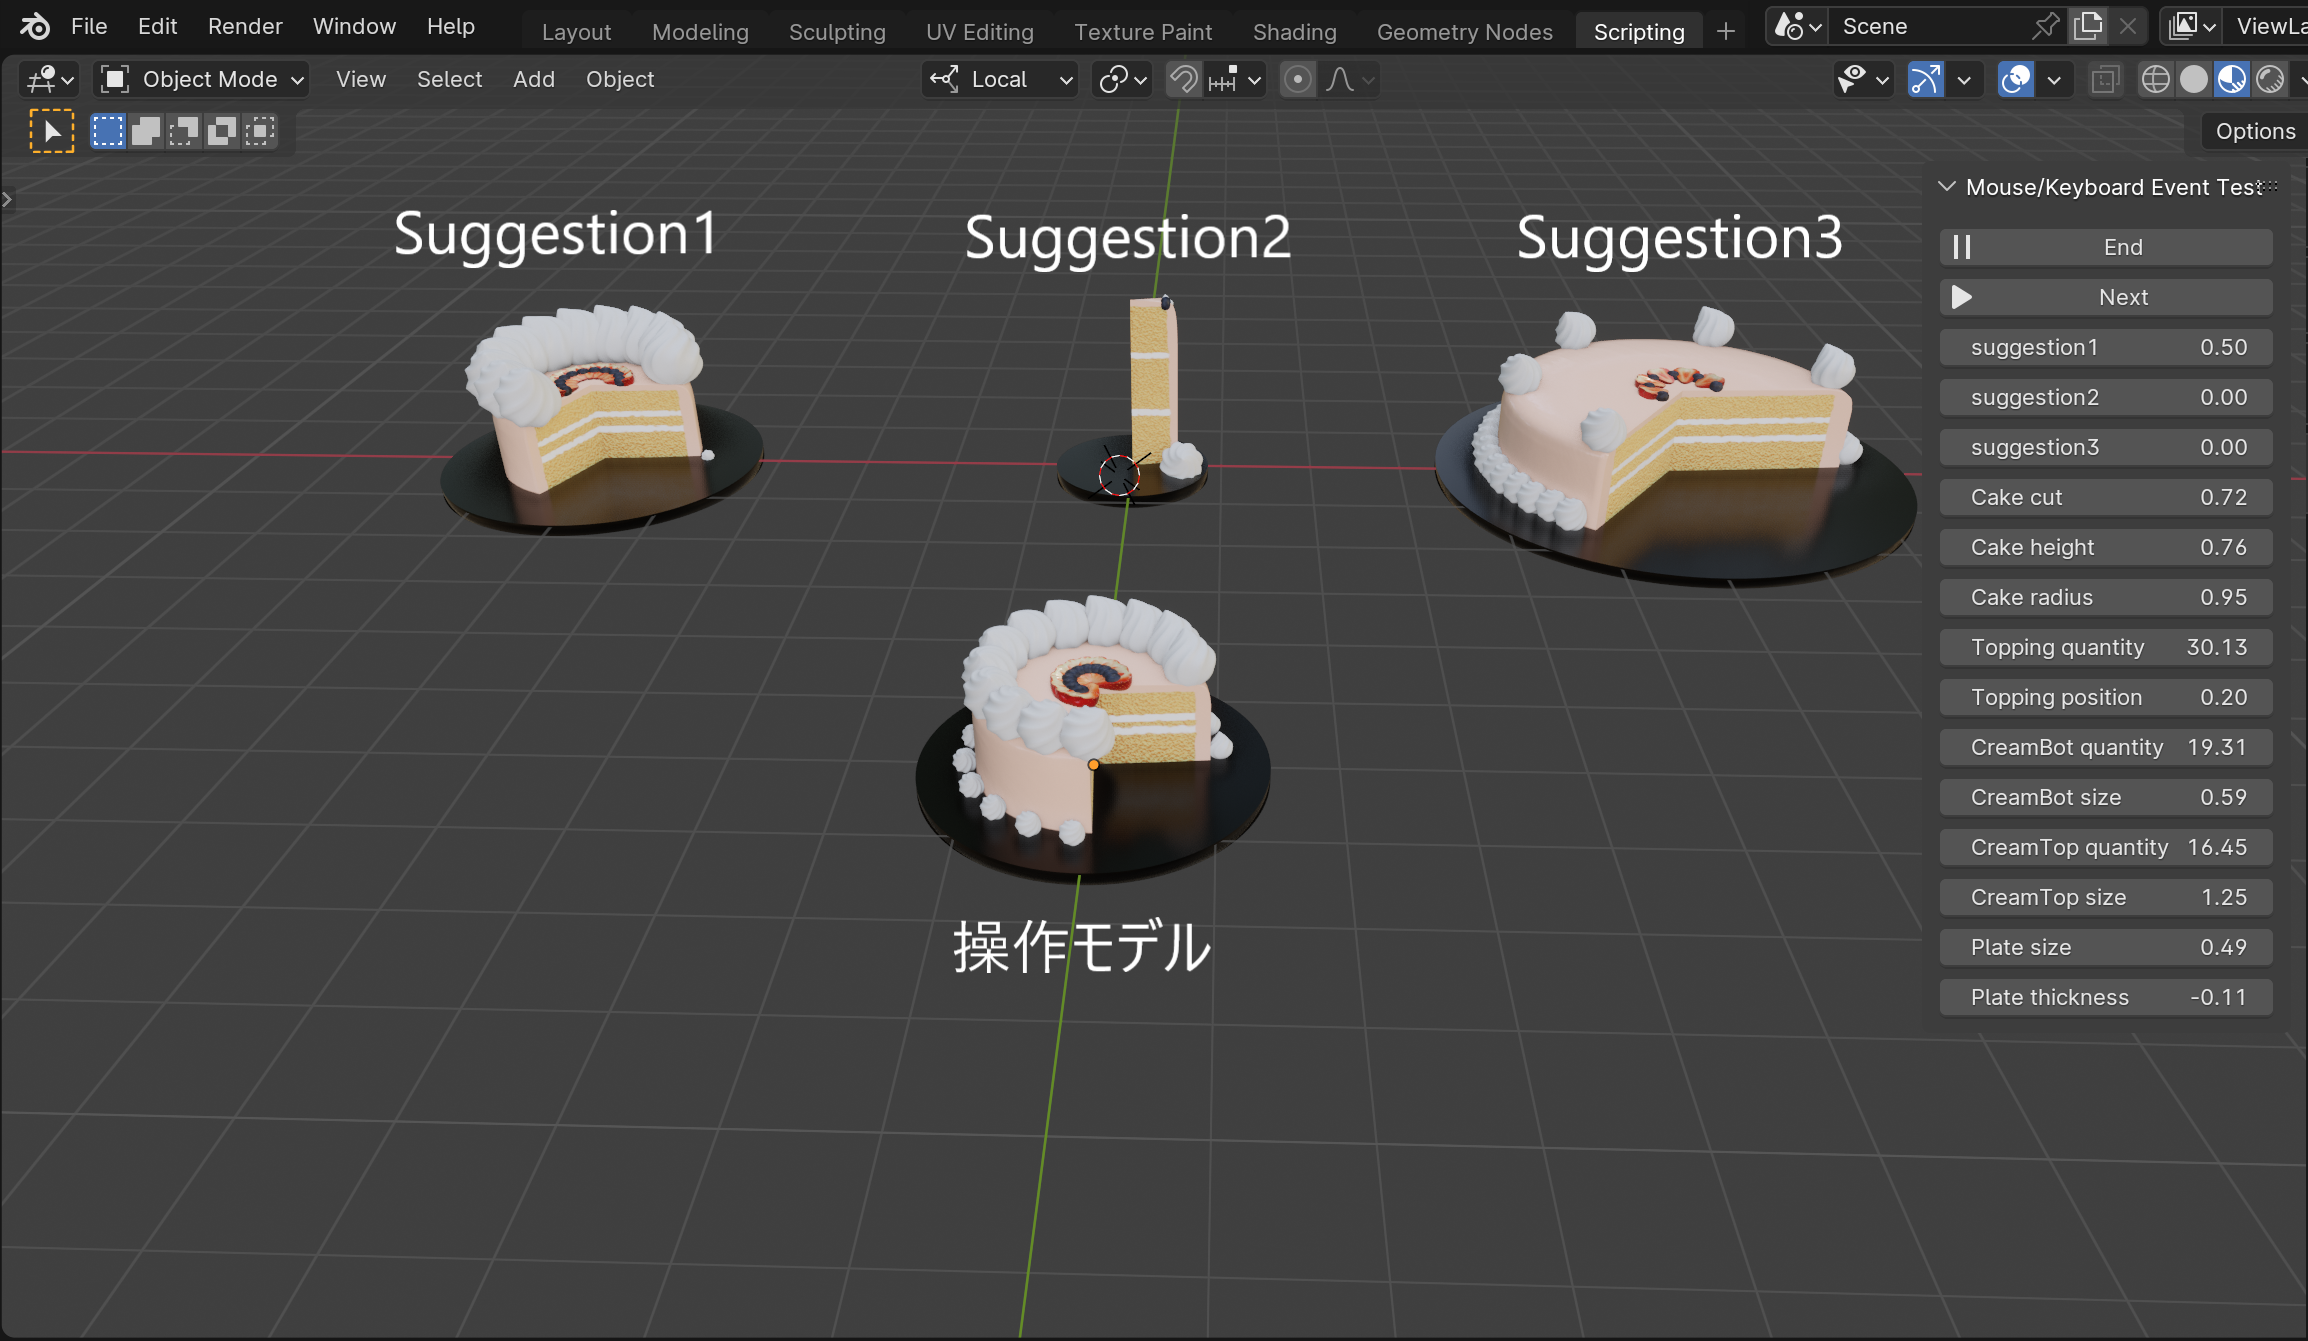
\includegraphics[scale=0.2]{./imgs/boAssistant2.png}
		\caption{BO as Assistant (Windows OSでの外観)\label{fig:boAssistant2}}
	\end{center}
\end{figure}
\newpage


\subsection{アンケート項目}
表\ref{tb:questions1},\ref{tb:questions2}に本実験で行うアンケート項目を示す.
アンケートの種類は提案システムに対する評価と,対照実験と比較した場合の評価の2種類である.
回答については5段階リッカート尺度\cite{likert1932technique}によって行う.
また選択回答に加えて,システムに関する良い点,不満点,感想についての自由記述も行う.

\begin{table}[h]
        \centering
	\caption{提案システムの使用感に関するアンケート(5段階評価)\label{tb:questions1}}
	\scalebox{1.0}{
		\begin{tabular}{|l|} \hline
                 1 : 使用方法について理解するには簡単であると感じましたか?\\ \\
                 2 : 使いやすいと感じましたか?\\ \\
                 3 : 操作時間は短いと感じましたか?\\ \\
                 4 : 操作する項目数は少ないと感じましたか?\\ \\
                 5 : モデルを広く探索できたと感じましたか?\\ \\
                 6 : 満足のいくモデリングが出来ましたか?\\ \\
                 7 : プロシージャルモデリングをするときに有用性があると感じましたか?\\ \\
                 8 : また本システムを使いたいと感じましたか?\\ \hline
		\end{tabular}
	}
\end{table}

\begin{table}[t]
        \centering
	\caption{対照実験との比較に関するアンケート(5段階評価)\label{tb:questions2}}
	\scalebox{1.0}{
		\begin{tabular}{|l|} \hline
                 9 : 目的のモデルが与えられた実験ではどちらの方が利用するのに適していると思いますか?\\ \\
                 10 : 自由にモデリングをした実験ではどちらの方が利用するのに適していると思いますか?\\ \\
                 11 : パラメータ数が少ないモデルではどちらの方が利用するのに適していると思いますか?\\ \\
                 12 : パラメータ数が多いモデルではどちらの方が利用するのに適していると思いますか?\\ \\
                 13 : モデリングにかかる時間はどちらの方が長いと感じましたか?\\ \\
                 14 : モデルの探索範囲はどちらの方が広いと感じましたか?\\ \\
                 15 :どちらのシステムが有用性が高かったですか
                 \\ \hline
		\end{tabular}
	}
\end{table}
\newpage


\subsection{実験の流れ}
本実験ではモデルのパラメータ数が実験1よりも実験2のほうが多いものを利用している関係上,実験2のタスクのほうが難度が高いものになっている.システム操作の理解が高い状態で難度の高いタスクを行ってもらうために,実験1の次に実験2を取り組みという手順で固定している.以下に,実験の順序を説明する.

\begin{enumerate}
    \item プロシージャルモデリングの簡単な説明
    \item 提案システム,対照実験用システムの説明および練習
    \item Cake モデルのパラメータ説明,動作確認
    \item 実験1
    \item Sofa モデルのパラメータ説明,動作確認
    \item 実験2
    \item アンケート回答
\end{enumerate}

\clearpage
\section{結果と考察}
\subsection{定性評価}
図\ref{fig:exp1TimeComp}にシステムの操作時間についての箱ひげ図を示す.表\ref{tb:exp1TimeComp}に各平均値,標準偏差を示す.時間の平均値に関して提案システムのほうが,既存システムよりも短縮されているようにも見えるが,図\ref{fig:exp1TimeComp}からも分かるように,既存システムでは大きな値に外れ値が存在するためであると考えられる.一方で,図\ref{fig:exp1AllTime}において提案システムのほうがばらつきが大きいことが分かる.この差について,システム理解における差ではないかと考えられる.実験の流れとして,実験の前にプロシージャルモデリングの各パラメータが何を示すのかを理解するために一度パラメータ操作をしてもらっており,既存システムではパラメータ操作に追加機能を実装する形のものである.そのため,システム操作の理解度が提案システムのほうが低かったために生じた差であると考えられる.


また,1ステップごとの提案モデルおよび決定したモデルの見本のモデルへの推移について,具体的なグラフは\hyperref[appendix:gaChange]{付録B}にて掲載する.結果として,システムが機能し収束していくデータもあれば,上手くいかないものもあった.これは IGA のランダム性の高さが寄与していると考えられる.



\begin{figure}[h]
 \begin{minipage}[b]{0.48\linewidth}
  \centering
  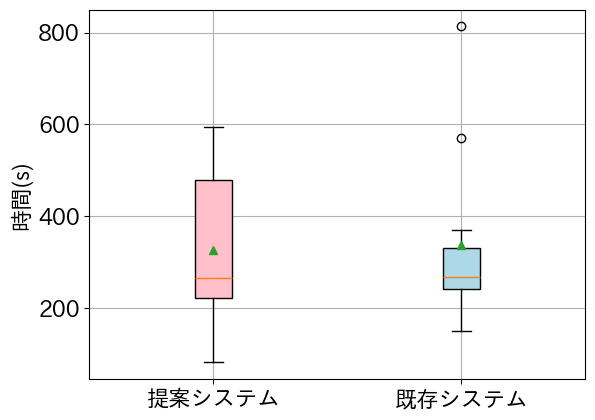
\includegraphics[scale=0.4]{./imgs/result/cakeAllTime.png}
        \subcaption{全時間}\label{fig:exp1AllTime}
 \end{minipage}
 \begin{minipage}[b]{0.48\linewidth}
  \centering
  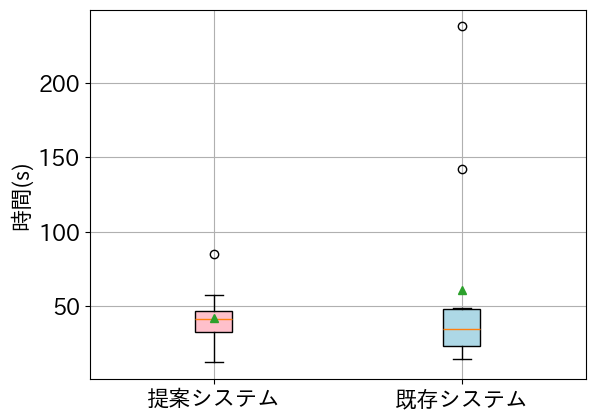
\includegraphics[scale=0.4]{./imgs/result/cakeStepTime.png}
        \subcaption{1ステップ当たりの時間}
 \end{minipage}\\
 \begin{minipage}[b]{0.48\linewidth}
  \centering
  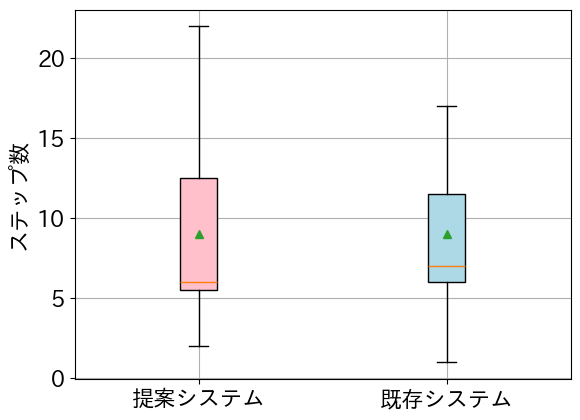
\includegraphics[scale=0.4]{./imgs/result/cakeStepCnt.png}
        \subcaption{ステップ数}
 \end{minipage}
 \caption{実験1における操作時間の比較}\label{fig:exp1TimeComp}
\end{figure}

\begin{table}[h]
	\centering
	\caption{実験1における操作時間の平均と標準偏差\label{tb:exp1TimeComp}}
		\begin{tabular}{|c|c|c|c|} \hline
                システム&&平均&標準偏差\\ \hline\hline
                \multirow{3}{*}{既存システム}&全時間&337.445 s&181.72 s \\ \cline{2-4}
                &1ステップ当たりの時間&61.004 s&65.144 s \\ \cline{2-4}
                &ステップ数&9.0000 回&4.8617 回 \\ \hline
                \multirow{3}{*}{提案システム}&全時間&326.39 s&171.22 s \\ \cline{2-4}
                &1ステップ当たりの時間&42.079 s&17.804 s \\ \cline{2-4}
                &ステップ数&9.0000 回&5.7525 回 \\ \hline
		\end{tabular}
\end{table}
\newpage

図\ref{fig:exp2TimeComp}にシステムの操作時間についての箱ひげ図を示す.表\ref{tb:exp2TimeComp}に各平均値,標準偏差を示す.図\label{fig:exp2AllTime}について,実験1よりも速い時間で終わっている.この原因としてはシステム操作への慣れと,実験1の終了判定の曖昧さの二つが考えられる.実験1の終了判定の曖昧さについて,終了基準は被験者本人の判断に任せているため,人によってはかなり厳密な調整を行っていた.一方で実験2でも終了条件自体は本人の基準ではあるが,実験1と違い見本画像がないため,より甘い基準で終了することが出来たためであると考えられる.

実験1同様に,1ステップごとの提案モデルおよび決定したモデルの見本のモデルへの推移について,具体的なグラフは\hyperref[appendix:gaChange]{付録B}にて掲載する.結果について,実験1とは反し,ランダム性によってステップ数が比較的短く終了したケースが多く存在する.一方で本システムとしては,4ステップで GA における一世代分に相当しているので GA としての収束機能が働かずに終わったということでもある.

\begin{figure}[h]
 \begin{minipage}[b]{0.48\linewidth}
  \centering
  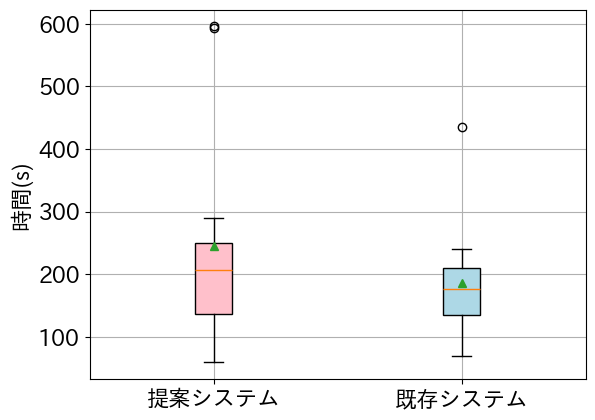
\includegraphics[scale=0.4]{./imgs/result/sofaAllTime.png}
        \subcaption{全時間}\label{fig:exp2AllTime}
 \end{minipage}
 \begin{minipage}[b]{0.48\linewidth}
  \centering
  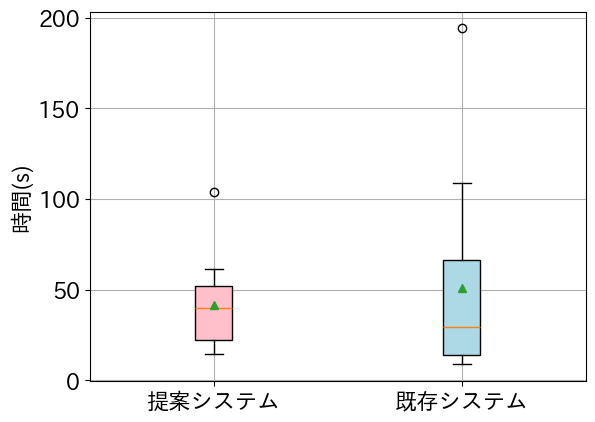
\includegraphics[scale=0.4]{./imgs/result/sofaStepTime.png}
        \subcaption{1ステップ当たりの時間}
 \end{minipage}\\
 \begin{minipage}[b]{0.48\linewidth}
  \centering
  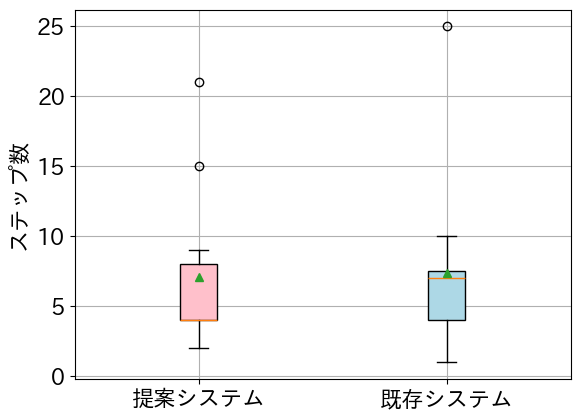
\includegraphics[scale=0.4]{./imgs/result/sofaStepCnt.png}
        \subcaption{ステップ数}
 \end{minipage}
 \caption{実験2における操作時間の比較}\label{fig:exp2TimeComp}
\end{figure}

\begin{table}[h]
	\centering
	\caption{実験2における操作時間の平均と標準偏差\label{tb:exp2TimeComp}}
		\begin{tabular}{|c|c|c|c|} \hline
                システム&&平均&標準偏差\\ \hline\hline
                \multirow{3}{*}{既存システム}&全時間&186.45 s&93.881 s \\ \cline{2-4}
                &1ステップ当たりの時間&51.136 s&56.049 s \\ \cline{2-4}
                &ステップ数&7.3636 回&6.1241 回 \\ \hline
                \multirow{3}{*}{提案システム}&全時間&245.70 s&175.30 s \\ \cline{2-4}
                &1ステップ当たりの時間&41.658 s&24.727 s \\ \cline{2-4}
                &ステップ数&7.0909 回&5.5996 回 \\ \hline
		\end{tabular}
\end{table}
\newpage


ここで表\ref{tb:paramTimeComp}に全体の操作時間のうち,個別のパラメータ調整をしている時間の比率を示す.
実験2の提案システムのものでは個別のパラメータ操作時間が非常に短いことが分かる.これは,個別パラメータを触らなかった被験者が8人いたからであり,明確な目的を持たずに動かす場合は提案システムの有効性が顕著であると考えられる.一方で既存システムでは全ての被験者が触れていた.これは既存システムのベイズ最適化の関係上,モデルに必要であると考えるパラメータを大きく動かさなければモデルの提案が滞ることと,常に操作できる位置に表示されていることが原因であると考えられる.
\begin{table}[h]
	\centering
	\caption{操作時間比率の平均と標準偏差\label{tb:paramTimeComp}}
		\begin{tabular}{|c|c|c|c|} \hline
                実験&システム&平均&標準偏差\\ \hline\hline
                \multirow{2}{*}{実験1}&既存システム&0.33493&0.14318 \\ \cline{2-4}
                &提案システム&0.24657& 0.17479 \\ \hline
                \multirow{2}{*}{実験2}&既存システム&0.41585&0.21003 \\ \cline{2-4}
                &提案システム&0.04111&0.07231 \\ \hline
		\end{tabular}
\end{table}
\newpage

その中で,図\ref{fig:tSNE_example}に t-SNE\cite{van2008visualizing} を用いてある被験者がシステムによって提案された Sofa モデルのパラメータを次元削減し可視化したものの一例を示す.全ての可視化図は\hyperref[appendix:tSNE]{付録C}に掲載する.
この散布図について縁取りが青いものが提案システム,赤いものが既存システムによる提案モデルであり,内部の色が0から1に行くにつれてステップ数が増加するようにしている.


提案システムのほうが既存システムの二倍のモデル提案を行うためプロット数自体は多い傾向にあるが,提案システムのほうがより広範囲の探索を行えているように見える.特に,既存システムにおいてより後のステップのもの同士が非常に近い位置にプロットされているのが確認できる.これはベイズ最適化によるモデル提案について,次の提案を行う直前に決定したモデルがそれまでに決定したモデルと大きく違うパラメータがあればそれをより再現しようとする方向に作用するためであり,収束率が高い一方でステップ数が大きくなるにつれ極端に探索範囲が狭まることに起因する.一方で提案システムのほうは多親交叉 REX によるランダム性があるため,ステップ間で見れば範囲は狭くなっているものの,多様性の保持が見られる.

\begin{figure}[h]
	\begin{center}
		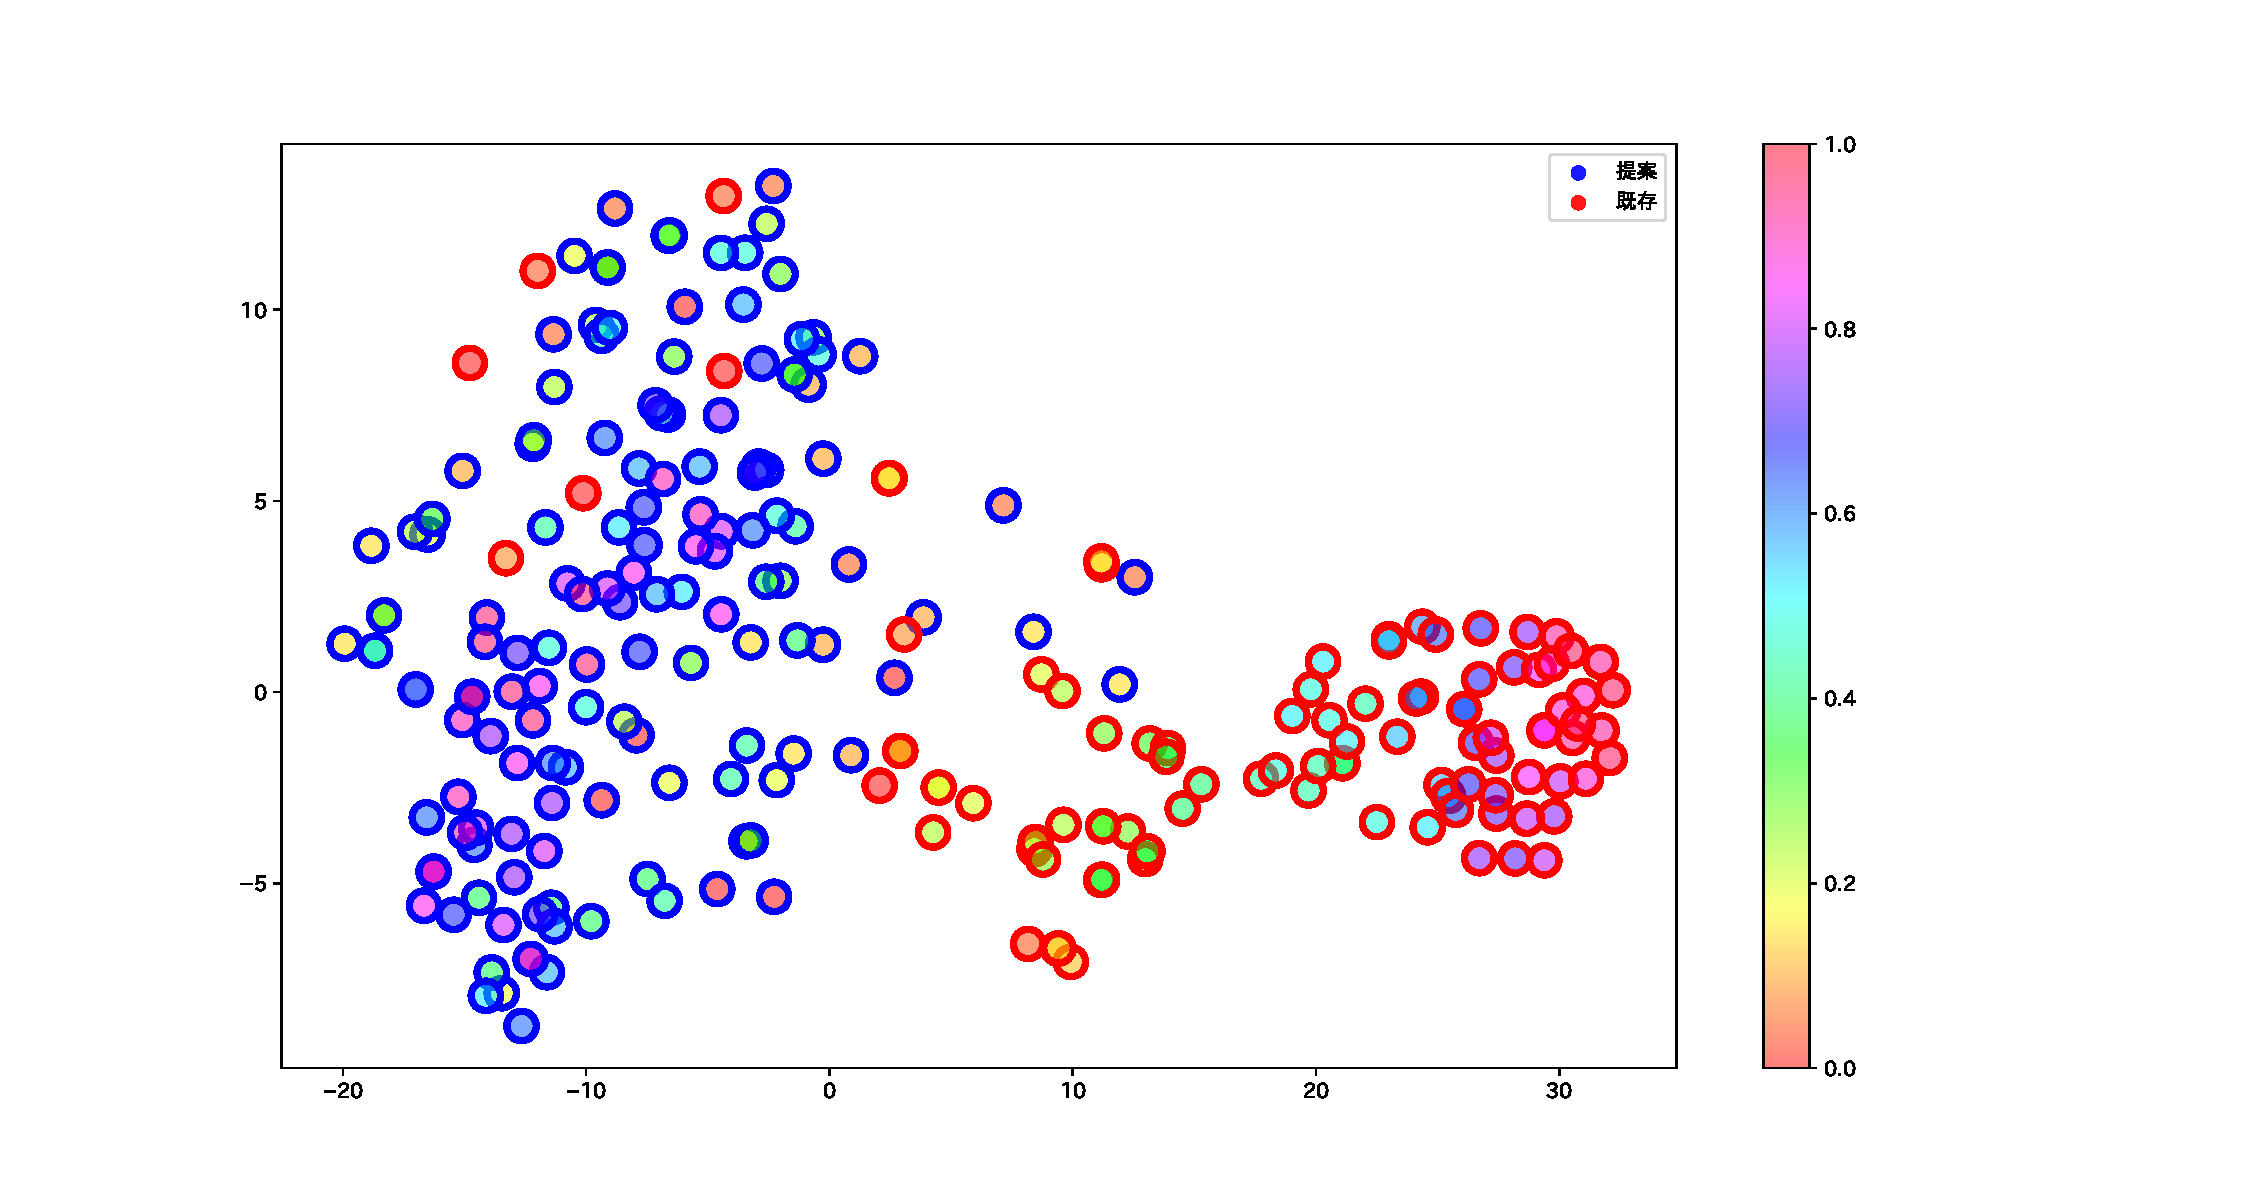
\includegraphics[scale=0.35]{./imgs/tSNE/sofa_5.pdf}
		\caption{提案された Sofa モデルのパラメータを二次元可視化した一例\label{fig:tSNE_example}}
	\end{center}
\end{figure}

\clearpage
\subsection{アンケート}

\subsubsection{選択}
図\ref{fig:questAns1},\ref{fig:questAns2}にアンケート結果を示す.図\ref{fig:questAns1}では1が negative, 5が positiveな評価であり,図\ref{fig:questAns2}では1が既存システム,5が提案システム寄りであることを示す.

まず提案システムの使用感について,全ての回答で平均が3を超えており,特にQ5-Q8については全て4を超えている.このことからシステム UI の方向性は間違っていないと考えられる.しかし,Q1の意見では良し悪しが分かれており,これは,ドラッグ操作と選択操作二種類がある点や,画面上に存在するモデルが計10個もあるという点によって分かりづらさがあったのではないかと考えられる.

次に対照実験との比較について,提案システムの優勢が高いと感じられたのはQ10,Q12,Q14であり,自由なモデリング,パラメータ数が多い時,探索範囲を広くしたい時にユーザの評価が高い.一方で,パラメータ数が少ないモデリング,操作時間については既存システムのほうが評価が高い.このことから,本システムはより複雑性の高いタスクに有効であり,簡単なモデリングであれば既存システムのほうが良い可能性がある.

\begin{figure}[h]
	\begin{center}
		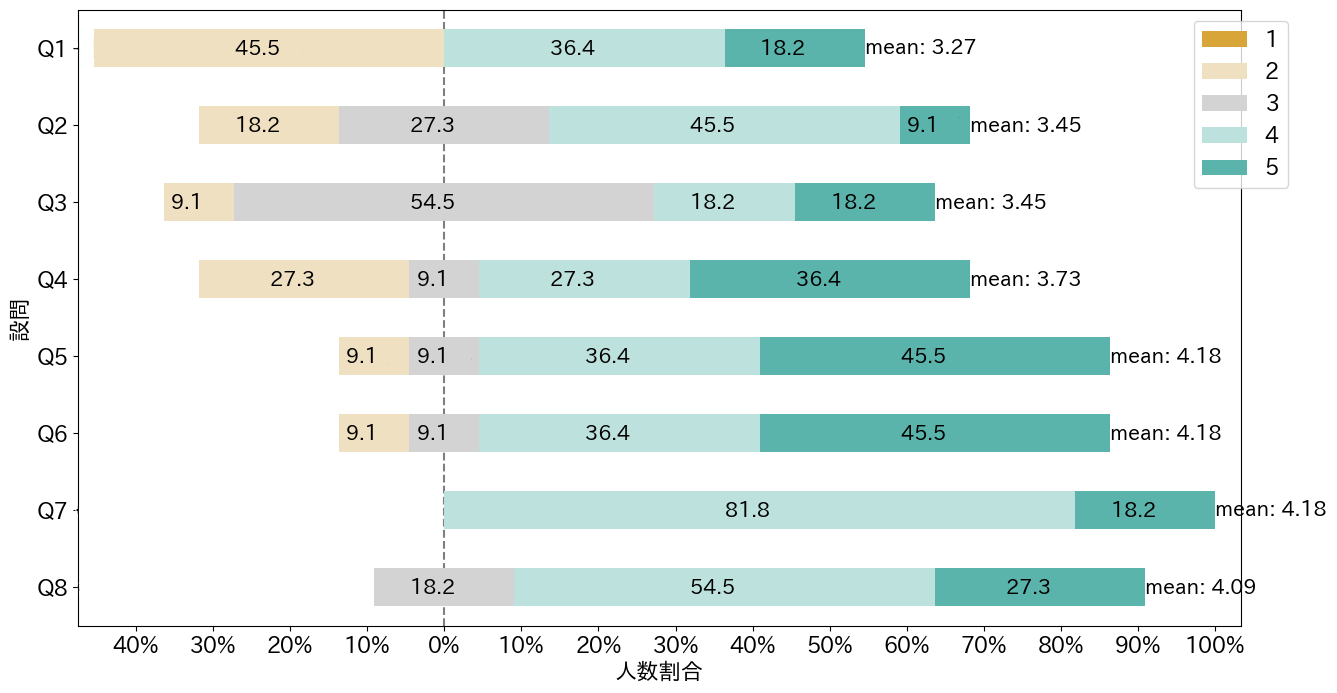
\includegraphics[scale=0.35]{./imgs/answer/questAns1.png}
		\caption{提案システムの使用感に関するアンケート結果\label{fig:questAns1}}
	\end{center}
\end{figure}

\begin{figure}[h]
	\begin{center}
		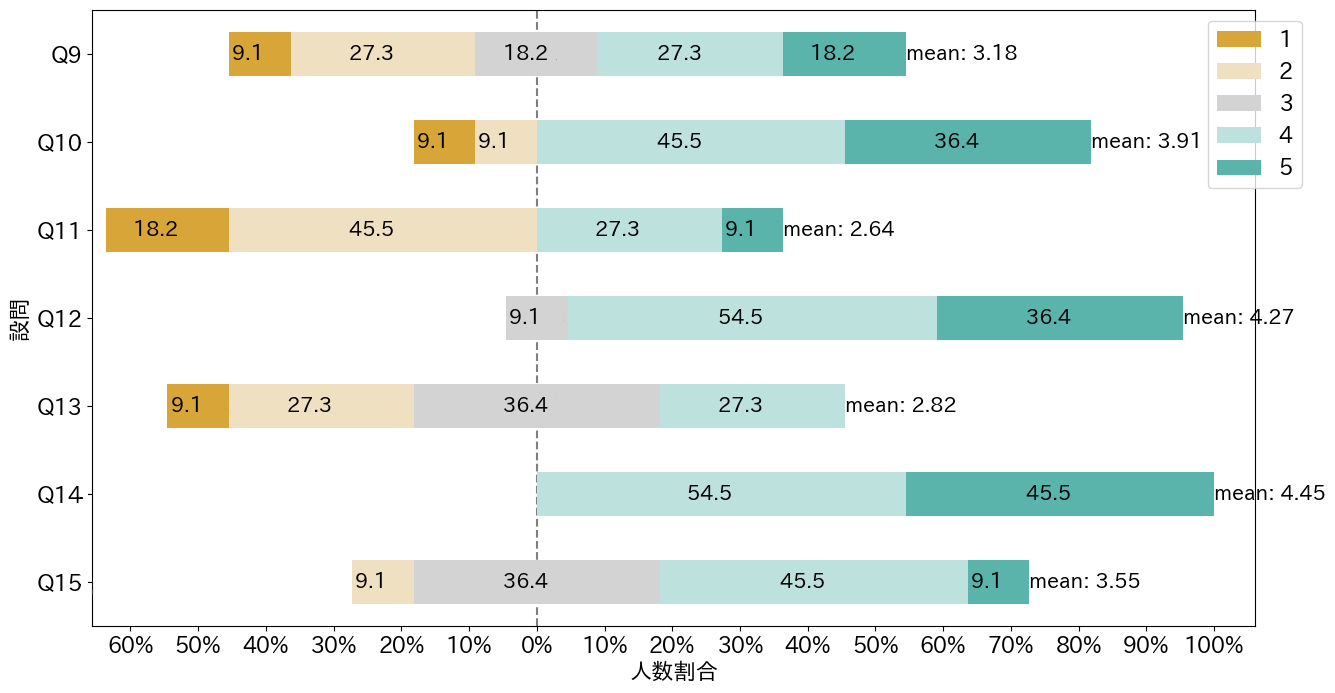
\includegraphics[scale=0.35]{./imgs/answer/questAns2.png}
		\caption{対照実験との比較に関するアンケート結果\label{fig:questAns2}}
	\end{center}
\end{figure}

\clearpage
\subsubsection{自由記述}
自由記述の回答について以下に示す.



\textbf{\underline{システムの良い点}}
\begin{enumerate}\label{en:systemGood}
    \item 新しいシステムは使いこなせれば大雑把に決めて、細かい部分だけ調整すれば完成できるため時間短縮になると感じました
    \item ソファでいう手すりの部分が欲しいというような理想を簡単にサイクルを回すことで再現することができる点が良いと思った。
    \item 自由にモデリングするパターンでは、パラメータの調整が直感的だった。
    \item 三角形の UI は直感的でわかりやすいとおもった
    \item 直感的で理解しやすかった.自由にモデリングをする実験では,自分が思いもよらないモデルができて良かったし,楽しかった.このシステムはパラメータが多くなるほど有用性が高まるように感じる.
    \item パラメータを動かしたときにモデルができるいろいろなパターンを先に見れることで、想像力が掻き立てられた
    \item 思いもよらないものができてくる点。とりあえず動かしてみて遊ぶことができる点。
    \item パラメータをが多いモデルはどれがどんな役割を持つのか把握しずらいため、ドラッグ操作のみで様々なモデルを探索できるのがとてもよかった。
    \item パラメータ調整でモデリングできたのはよかった
    \item 細かい操作をしなくても、システムがリコメンドしてくれて、形がそれっぽくなるのが楽だった
\end{enumerate}





\textbf{\underline{システムの悪い点}}
\begin{enumerate}
    \item 三角形の角に合わせて選択するやつが、左角から順番に選ばないといけないのが直感的には使いにくかったです
    \item 凝り性の人は、かなり時間がかかるかもしれないと感じた
    \item 赤い点の判定がもう少し広い方がよかったです。欲しいパーツが出てこないことがあり、直接パラメータを調整しなければいけない場合があった。
    \item 1個(例えばクリームの見た目)について近づけようとモデルを選んでいるといつの間にか他のが全然違くなっていることがあって難しいと感じた
    \item 最終的にディテールを突き詰める部分は,パラメータを調整する必要があると感じた.
    \item 目標が明確な時に、それから遠ざかるような選択肢しかない時がもどかしい
    \item 最初に選んだ三つのモデルから良いなと思ったモデルができたとき、次に新しい三つを選ぶとそれが消えてしまった。前段階で作成したモデル+新しい提案との組み合わせができるとよいなと思いました
    \item 最初に提案されるモデルの方向性を指定できると更に楽だと思いました
\end{enumerate}





\textbf{\underline{システムのその他感想}}
\begin{enumerate}
    \item 三角形の操作について理解するのに時間がかかった
    \item 時間制限が設けてある場合に使用するとかなり効果があるシステムだと感じた
    \item 大雑把な調整(概形)を提案システムで行って、細かい調整ができないパラメータ(整数のやつ)を最後に仕上げでいじるのが使いやすいのかなと思った
    \item 大雑把に形を作る際は,提案システムを利用することで,既存システムを利用するよりも早く完成させることができると感じた.
    \item 携帯のアプリケーションにしたら面白そう
    \item 後半になればなるほど、ここだけピンポイントで直したいということが多い
    \item 趣味で 3D モデリングをたしなんでいますが、システムから提案された複数のモデルを組み合わせる手法は、自身の発想からはみ出したアイデアを作品に組み込むことができてとても面白いなと思いました。
    \item 実用性は無いかもしれませんが、もっと色々なものが候補に出て、混ぜるとそれっぽくなるのは見てみたいです
    \item ランダムセレクトの因子が欲しかった。3要素のうちひとつめは、現在の最新モデルに固定してもよかったと思う(それまでの作業がキャンセルされてしまうため)
\end{enumerate}


システムの良い点としては UI の補間操作でドラッグによる直感的である点と,パラメータを同時に動かせることによって広く,おおまかな探索が出来る点が評価された.反対に悪い点としては,UIの操作性の悪さと,IGAによるランダム性が悪い方向に作用してユーザが良くないと思う方向へのモデル提案が行われてしまった点,細かい調整が提案システムだけでは難しい点が挙げられた.

\clearpage
\subsection{評価結果まとめ}
提案システムとしては,提案のランダム性および平面UIによる補間システムによって非常に幅広い探索が出来るシステムになったことが確かめられた.その一方で,本来の目的としていた時間短縮に関しては既存システムに対して優位性が見られなかった.ただし,ステップ数および操作時間に関して同等程度の結果である反面,広い探索を行えたという点に注目すれば探索についてのユーザビリティ向上は行えたと考えられる.

多くのパラメータを持つモデリングでは個別にパラメータが動かせる状況であれば,それに頼ることが多くなる.その結果Q12にみられるようにパラメータの多いモデリングでは提案システムに高い有効性があると考えられる.以上から,提案システムにおける UI は操作時間こそ減らすことは出来なかったものの,プロシージャルモデリングにおいて有効性が高いと考えられる.


一方で,遺伝的アルゴリズムによるモデル提案については上手く機能していると言い難く,実験2のように明確な目的がなければ,現状の UI だけで事足りてしまうことが多かった.そのため,明確な目的があれば収束する方向に,そうでなければ現在の操作モデルから大きく離れたモデルを提案する事でよりモデリング時の新しい発想が生まれて,洗練されたモデリングになっていくのではと考えられる.